\documentclass[12pt]{article}
\usepackage[utf8]{inputenc}
\usepackage[brazil]{babel}
\usepackage{graphicx}
\usepackage{geometry}
\usepackage{setspace}
\geometry{a4paper, margin=1in}
\usepackage[hyphens]{url}
\usepackage[hidelinks]{hyperref}  
\usepackage{float}

\begin{document}

\begin{center}
\textbf{RELATÓRIO TÉCNICO}
\end{center}

\noindent\textbf{DISCIPLINA:} Estatística e Probabilidade \\
\noindent\textbf{TURMA:} 4º B \\
\noindent\textbf{ALUNOS:} Thiago Queiroz e Julia Sales \\
\noindent\textbf{PROFESSOR:} Guilherme \\
\noindent\textbf{TEMA:} Análise Estatística de Pets no Jogo Pet Simulator 99 \\

\doublespacing

\section*{1. INTRODUÇÃO}

Este relatório apresenta uma análise estatística e probabilística com base nos dados de pets do jogo Pet Simulator 99 (PS99), obtidos por meio da API oficial do jogo e armazenados nos arquivos"pets\_data.json" e "rap\_data.json". A base de dados contempla informações relevantes como identificação dos pets, raridade (Normal, Golden ou Rainbow), status shiny (valor booleano), tamanho(Normal, Huge, Titanic e Gargantuan), quantidade existente e valor estimado em diamantes (Também referido como "RAP", dentro do jogo).

O objetivo principal desta análise é aplicar conceitos fundamentais de Estatística e Probabilidade, incluindo: probabilidade simples, união, interseção, complemento, probabilidade condicional e o Teorema de Bayes. Além disso, abordam-se definições de variáveis aleatórias, funções de probabilidade e de repartição, bem como medidas estatísticas como variância, desvio padrão, covariância e correlação. Gráficos foram elaborados para auxiliar na visualização dos dados, e cada etapa analítica é devidamente justificada para reforçar sua relevância na compreensão do conjunto de dados.

O tema escolhido — o jogo \textit{Pet Simulator 99}, disponível na plataforma Roblox — foi selecionado por seu potencial analítico e sua complexa dinâmica econômica. O jogo consiste na coleta e evolução de pets, que possuem níveis distintos de força. Em sua forma base, a hierarquia de força segue a ordem: Pets Normais \textless{} Pets Huge \textless{} Pets Titanic \textless{} pets Gargantuan. Cada pet pode ainda possuir variações de raridade (Normal \textless{} Golden \textless{} Rainbow) e o status shiny, que atuam como multiplicadores adicionais de força.

A escolha deste tema se justifica pela complexidade da economia dentro do jogo, que opera com base em um sistema de mercado livre. Os jogadores têm autonomia para definir os preços dos itens disponíveis para troca, podendo comprar ou vender livremente conforme seus próprios critérios de valor, sem a imposição de restrições significativas. Esse ambiente fornece um rico contexto para a aplicação de técnicas estatísticas e probabilísticas, permitindo análises que simulam cenários reais de mercado com variáveis diversas.

\section*{2. METODOLOGIA}
Os dados foram processados no Google Colab utilizando Python, com bibliotecas como pandas, numpy, matplotlib e seaborn. Os arquivos JSON foram carregados, tratados e mesclados em um único DataFrame com colunas como "Id", "Raridade", "Shiny", "Tamanho", "Existe" (quantidade existente) e "Valor" (em diamantes). Funções foram criadas para filtrar e contar pets com base em critérios específicos, como tamanho e raridade. Probabilidades foram calculadas com base na quantidade total de pets existentes, e gráficos foram gerados para ilustrar distribuições e relações. Medidas estatísticas foram computadas para variáveis numéricas e categóricas, com justificativas para cada escolha analítica.

\section*{3. DESENVOLVIMENTO}

\subsection*{3.1 Probabilidade Simples}
\begin{itemize}
    \item P(Pet ser Huge): 0.00012\%
    \item P(Pet ser Titanic): 0.00000044\%
    \item P(Pet ser Gargantuan): 0.0000000022\%
\end{itemize}
\textbf{\textit{Justificativa}}: Essas probabilidades foram calculadas para avaliar a raridade dos pets mais desejados do jogo (Huge, Titanic e Gargantuan), que são de interesse dos jogadores por seu alto valor e status. A análise ajuda a entender a distribuição de pets raros, que se mostrou extremamente baixa.

\subsection*{3.2 Probabilidade com União}
\begin{itemize}
    \item P(Golden ou Rainbow): 22.60%\%
    \item P(Huge ou Shiny): 0.50 \%
    \item P(Titanic ou Valor $>$ 100M): 0.00456\%
\end{itemize}
\textbf{\textit{Justificativa}}: A probabilidade com união foi usada para analisar a chance de um pet possuir características desejáveis combinadas, como raridade (Golden ou Rainbow) ou atributos de tamanho e aparência (Huge ou Shiny).

Também foi analisado que há baixa chance de certo pet ser caro ou de uma raridade superior no jogo, o que faz sentido pois a maioria dos pets existentes são normais e sem multiplicadores, fazendo que o preço seja mais baixo. Isso é relevante para jogadores que buscam pets com múltiplas qualidades, refletindo cenários reais de decisão no jogo.

\subsection*{3.3 Probabilidade com Intersecção}
\begin{itemize}
    \item P(Gargantuan e Rainbow e Shiny): 0.000000000003413\%
    \item P(Huge e Valor $\leq$ 30M): 54.17\%
    \item P(Titanic e Valor $\geq$ 20B): 15.10\%
\end{itemize}
\textbf{\textit{Justificativa}}: A operação de interseção foi empregada com o objetivo de identificar a probabilidade de ocorrência simultânea de características específicas em pets, como no caso do denominado "melhor pet possível" — aquele que apresenta as combinações Gargantuan, Rainbow e Shiny — cuja probabilidade de obtenção é extremamente baixa, beirando a impossibilidade estatística.

Adicionalmente, verificou-se que uma parcela significativa dos pets da categoria Huge é classificada como de baixo valor, possivelmente em função da elevada quantidade de cópias existentes de determinados exemplares, o que contribui para a redução de seus preços.
Em contraste, observou-se que uma proporção considerável dos pets da categoria Titanic possui valores superiores a 20 bilhões (20B), tornando-os economicamente inviáveis para a maioria dos jogadores.

Tais informações são úteis para avaliar a viabilidade de encontrar pets com condições específicas, importante para planejamento no jogo.

\subsection*{3.4 Probabilidade com Complemento/Diferença}
\begin{itemize}
    \item P(Não Shiny): 99.50038\%
    \item P(Não Huge): 99.99988\%
    \item P(Titanic, mas não Golden): 90.58\%
\end{itemize}
\textbf{\textit{Justificativa}}: O uso do complemento ajuda a entender a probabilidade de ausência de características desejáveis (como não ser Shiny ou Huge), enquanto a diferença (Titanic, mas não Golden) avalia exclusões específicas. Essas métricas são úteis para jogadores que querem evitar certos tipos de pets com algum multiplicador específico (No caso Shiny, Huge e Golden), visto que normalmente são menos em conta, ou focar em categorias específicas.   

\subsection*{3.5 Probabilidade Condicional}
\begin{itemize}
    \item P(Shiny $|$ Rainbow):  1.02\%
    \item P(Shiny $|$ Titanic): 1.80\%
    \item P(Valor $>$ 1B $|$ Huge): 0.48\%
\end{itemize}
\textbf{\textit{Justificativa}}: A probabilidade condicional foi utilizada para analisar a dependência entre características, como a chance de um pet Rainbow ser Shiny (O que normalmente é o pet mais forte da maioria dos jogadores de longa data) ou de um Huge ter alto valor (O que significa que ele provavelmente tem uma aparência desejável).
Também foi analisado que em todas categorias é improvável que ambas características aconteçam, o que faz sentido com a realidade do jogo, pois é mais difícil conseguir um pet Rainbow e/ou Shiny, independente de seu tamanho e um Huge ter valor maior que 1B indica que ele é raro e por consequência, poucos tem um valor demasiadamente alto.

Isso reflete cenários no jogo onde jogadores avaliam a probabilidade de uma característica dado que outra já está presente, auxiliando na tomada de decisões.

\subsection*{3.6 Probabilidade com Teorema de Bayes}
\begin{itemize}
    \item P(Titanic $|$ Valor $>$ 50M): 0.0029\%
    \item P(Shiny $|$ Golden): 0.73\%
    \item P(Normal e Não Shiny $|$ Valor $<$ 30M): 99.50\%
\end{itemize} 
\textbf{\textit{Justificativa}}:  O Teorema de Bayes foi aplicado para inverter relações condicionais, como a chance de um pet ser da categoria Titanic dado que possui alto valor de mercado. Essa abordagem é importante para jogadores que, ao se depararem com um pet caro, desejam estimar a probabilidade de ele pertencer a uma categoria específica. Com isso, é possível tomar melhores decisões em relação a aquisição de determinados pets.   

Por exemplo, ao considerar a probabilidade de um pet ser Shiny dado que é Golden, ou ser do tipo Normal e não Shiny considerando um valor de mercado inferior a 30 milhões, é possível entender melhor a distribuição e frequência real dessas combinações no universo do jogo.

Os resultados obtidos demonstram que, mesmo diante de características que poderiam sugerir maior raridade (como um valor elevado), a ocorrência efetiva de categorias extremamente raras, como Titanic ou Shiny, permanece estatisticamente baixa. 

\subsection*{3.7 Definição de Novas Variáveis Aleatórias}
\begin{itemize}
    \item \textbf{X\_tamanho}: Numérica discreta, representando o tamanho do pet (Normal = 0, Huge = 1, Titanic = 2, Gargantuan = 3).
    \item \textbf{Y\_shiny}: Binária, indicando se o pet é shiny (Não Shiny = 0, Shiny = 1).
\end{itemize}
\textbf{\textit{Justificativa}}: Essas variáveis foram criadas para transformar atributos categóricos em numéricos, permitindo cálculos probabilísticos e estatísticos como funções de probabilidade e repartição. O tamanho e o status shiny são características centrais no jogo, impactando principalmente valor e o multiplicador de dano.

\subsection*{3.8 Função de Probabilidade}
\begin{itemize}
    \item \textbf{X\_tamanho}:
    \begin{itemize}
        \item P(X = 0) = 0.999998815627
        \item P(X = 1) = 0.000001179907
        \item P(X = 2) = 0.000000004444
        \item P(X = 3) = 0.000000000022
    \end{itemize}
    \item \textbf{Y\_shiny}:
    \begin{itemize}
        \item P(Y = 0) = 0.99500
        \item P(Y = 1) = 0.00500
    \end{itemize}
\end{itemize}
\textbf{\textit{Justificativa}}: As funções de probabilidade foram definidas para descrever a distribuição de probabilidade das variáveis X\_tamanho e Y\_shiny, permitindo uma visão clara da frequência relativa de cada categoria.
Nessa análise foi reforçado algo que já era aparente antes: Pets não normais são extremamente incomuns, o que é fundamental para entender a composição geral dos pets no jogo.

\subsection*{3.9 Função de Repartição (Cumulativa)}
\begin{itemize}
    \item \textbf{F(X $\leq$ x)} (X\_tamanho):
    \begin{itemize}
        \item F(X $\leq$ 0) = 0.999998815627
        \item F(X $\leq$ 1) = 0.999999995534
        \item F(X $\leq$ 2) = 0.999999999978
        \item F(X $\leq$ 3) = 1.000000000000
    \end{itemize}
    \item \textbf{F(Y $\leq$ y)} (Y\_shiny):
    \begin{itemize}
        \item F(Y $\leq$ 0) = 0.99500
        \item F(Y $\leq$ 1) = 1.00000
    \end{itemize}
\end{itemize}
\textbf{\textit{Justificativa}}: As funções de repartição foram calculadas para mostrar a probabilidade acumulada de cada variável, permitindo uma análise da probabilidade de um pet ter um tamanho ou status shiny até certo ponto. Isso é útil para prever a chance de encontrar pets com características específicas.

\subsection*{3.10 Gráficos}
\begin{itemize}
    \item \textbf{Gráfico 1}: Barras da quantidade de pets existentes por raridade (Normal, Golden, Rainbow).
     \begin{figure}[H]
         \centering
         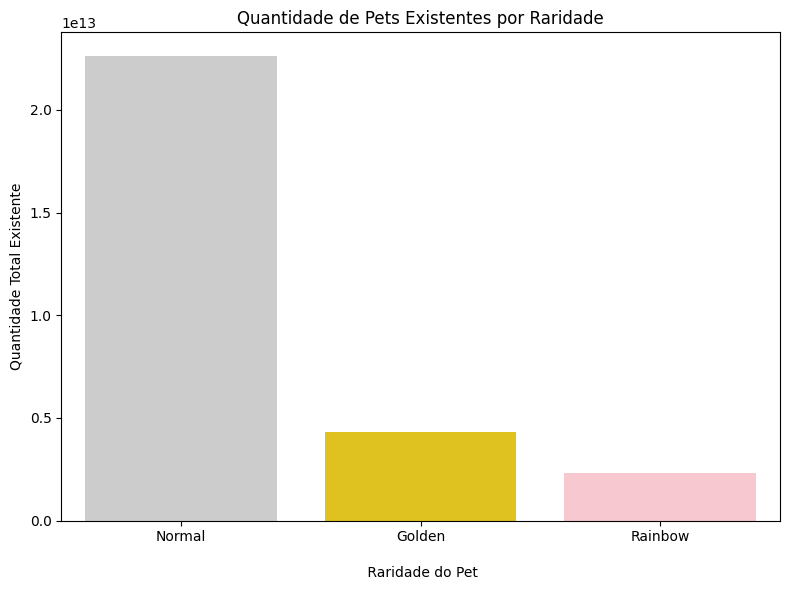
\includegraphics[width=0.8\textwidth]{grafico1.png}
         \caption{Quantidade de Pets Existentes por Raridade}
     \end{figure}
    \item \textbf{Gráfico 2}: Pizza da proporção de pets shiny vs. não shiny (baseado em existentes).
     \begin{figure}[H]
         \centering
         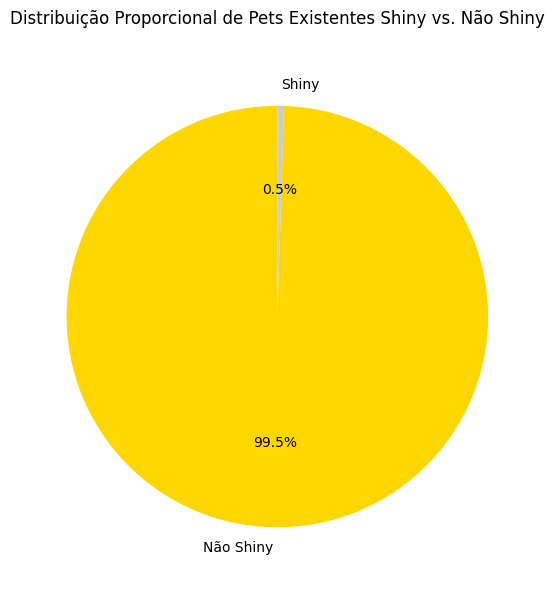
\includegraphics[width=0.8\textwidth]{grafico2.png}
         \caption{Distribuição Proporcional de Pets Existentes Shiny vs. Não Shiny}
     \end{figure}
    \item \textbf{Gráfico 3}: Dispersão do valor dos pets vs. quantidade existente (escalas logarítmicas).
     \begin{figure}[H]
         \centering
         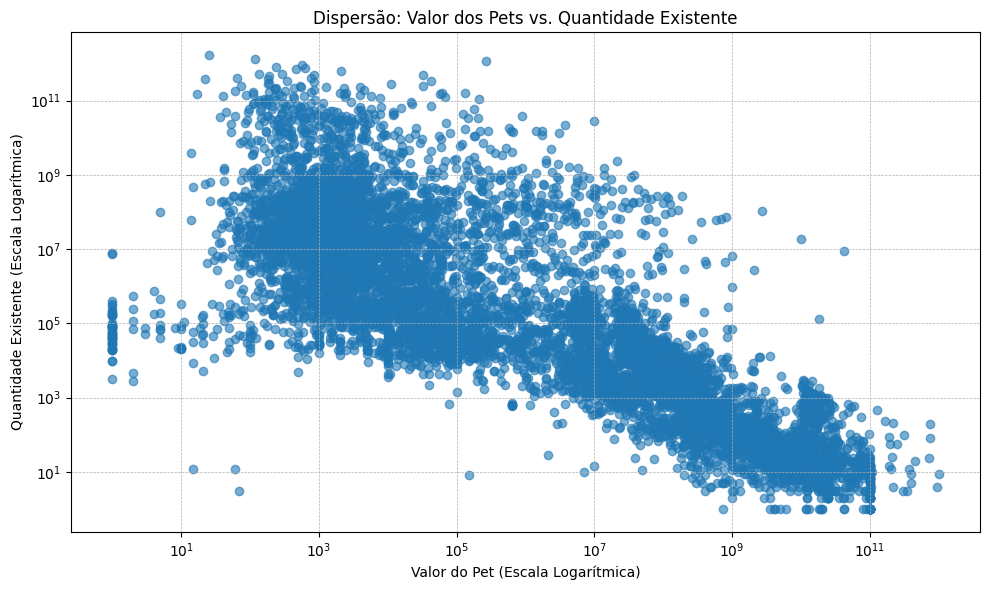
\includegraphics[width=0.8\textwidth]{grafico3.png}
         \caption{Dispersão: Valor dos Pets vs. Quantidade Existente}
     \end{figure}
    \item \textbf{Gráfico 4}: Barras da frequência de pets únicos por tamanho (Normal, Huge, Titanic, Gargantuan).
     \begin{figure}[H]
         \centering
         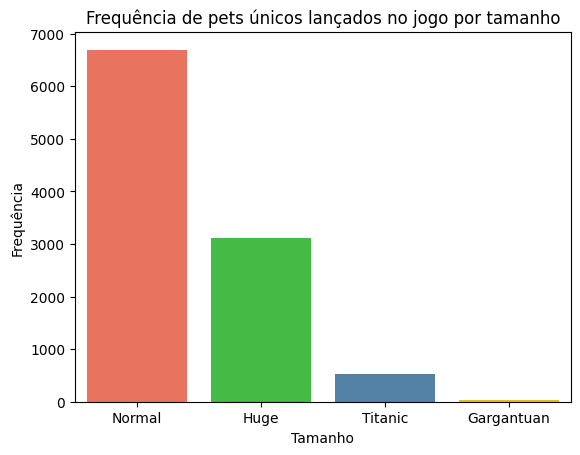
\includegraphics[width=0.8\textwidth]{grafico4.png}
         \caption{Frequência de Pets Únicos Lançados no Jogo por Tamanho}
     \end{figure}
    \item \textbf{Gráfico 5}: Barras da quantidade absoluta de pets shiny vs. não shiny (baseado em existentes).
     \begin{figure}[H]
         \centering
         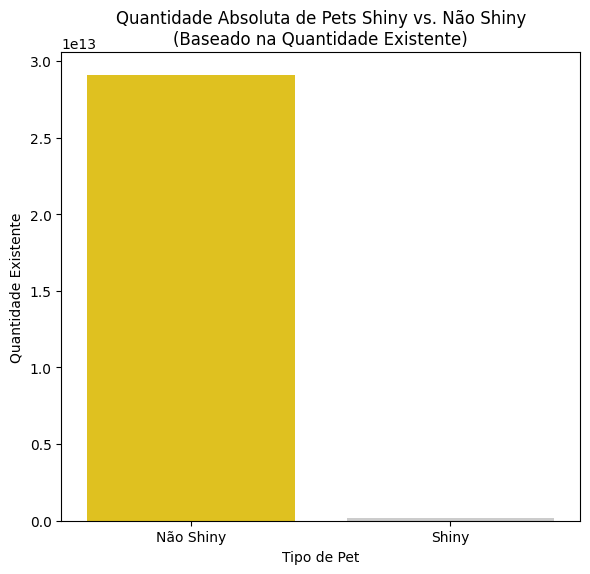
\includegraphics[width=0.8\textwidth]{grafico5.png}
         \caption{Quantidade Absoluta de Pets Shiny vs. Não Shiny}
     \end{figure}   
\end{itemize}
\textbf{\textit{Justificativa}}: Os gráficos foram selecionados com o propósito de representar visualmente as distribuições de atributos (raridade, status \textit{shiny} e tamanho), bem como analisar relações quantitativas, como entre valor de mercado e quantidade existente. Essas visualizações permitem a identificação de padrões relevantes, tais como a predominância de pets na forma Normal (sem multiplicadores) em comparação com suas variações Golden, Rainbow e Shiny; a baixa frequência de lançamento de pets das categorias Titanic e Gargantuan; e a relação inversamente proporcional entre valor e quantidade existente, evidenciando a tendência de que pets com menor disponibilidade apresentam preços significativamente mais elevados.

\subsection*{3.11 Variância e Desvio Padrão}
\begin{itemize}
    \item \textbf{Quantidade Existente por Tamanho}:
    \begin{itemize}
        \item Variância: 1.61E+26
        \item Desvio Padrão: 1.27E+13
    \end{itemize}
\end{itemize}
\textbf{\textit{Justificativa}}: A variância e o desvio padrão foram calculados para medir a dispersão da quantidade existente e do valor dos pets. Isso é importante para entender a variabilidade entre diferentes tamanhos e valores, indicando o quão heterogêneo é o conjunto de pets no jogo. O motivo dessa heterogeneidade se dá por fatores como dados muito espalhados em torno da média e valores extremos (outliers) influenciando a distribuição.

\subsection*{3.12 Covariância}
\begin{itemize}
    \item \textbf{Valor-Raridade}: 8.08E+8
    \item \textbf{Valor-Tamanho}: 8.0816E+8
\end{itemize}
\textbf{\textit{Justificativa}}: A covariância foi usada para avaliar a relação linear entre valor e outras variáveis (raridade e tamanho). Valores positivos indicam que pets mais raros ou maiores tendem a ter maior valor, o que é esperado no contexto do jogo e útil para estratégias de compra e revenda de pets.

\subsection*{3.13 Correlação}
\begin{itemize}
    \item \textbf{Valor-Raridade}: 0.04
    \item \textbf{Valor-Tamanho}: 0.30
\end{itemize}
\textbf{\textit{Justificativa}}: A correlação foi calculada para quantificar a força da relação entre valor e as variáveis raridade e tamanho. Os valores positivos, embora baixos, confirmam uma associação fraca, mas existente, entre maior raridade/tamanho e maior valor, fornecendo insights sobre o mercado de pets no jogo.

\section*{4. CONCLUSÃO}
Neste trabalho, utilizamos dados reais extraídos da API do jogo Pet Simulator 99 para aplicar conceitos de Probabilidade e Estatística. Através da categorização dos pets por raridade, tamanho e se é shiny ou não, realizamos análises que incluíram distribuição de frequência, cálculo de probabilidades e distribuições cumulativas.

Para concluir, foi visto que a maioria dos pets presentes no jogo são do tipo "Normal" (cerca de 99\%), enquanto pets "Golden", "Rainbow" e "Shiny" são significativamente mais raros. Além disso, os tamanhos "Huge", "Titanic" e "Gargantuan" representam uma minoria, reforçando o valor estatístico e comercial desses pets no jogo. As análises também mostraram que a chance de obter um pet shiny de qualquer tipo é aproximadamente 0.5\%, demonstrando sua exclusividade. A distribuição cumulativa reforçou essas conclusões ao evidenciar a baixa incidência de pets raros.

Todas as escolhas analíticas foram justificadas para atender aos objetivos da análise, fornecendo uma visão estatística abrangente dos pets no PS99.

\section*{5. REFERÊNCIAS}
\section*{Referências}

\begin{itemize}
  \item PET SIMULATOR WIKI. \textit{List of Pets (Pet Simulator 99)}. Disponível em: \url{https://pet-simulator.fandom.com/wiki/List_of_Pets_(Pet_Simulator_99)}. 

  \item PET SIMULATOR WIKI. \textit{Huge Pets (Pet Simulator 99)}. Disponível em: \url{https://pet-simulator.fandom.com/wiki/Huge_Pets_(Pet_Simulator_99)}. 

  \item PET SIMULATOR WIKI. \textit{Titanic Pets (Pet Simulator 99)}. Disponível em: \url{https://pet-simulator.fandom.com/wiki/Titanic_Pets_(Pet_Simulator_99)}.  2025.

  \item PET SIMULATOR WIKI. \textit{Gargantuan Pets (Pet Simulator 99)}. Disponível em: \url{https://pet-simulator.fandom.com/wiki/Gargantuan_Pets_(Pet_Simulator_99)}.

  \item PS99 RAP. \textit{Pet Simulator 99 RAP Database}. Disponível em: \url{https://ps99rap.com}. 

  \item Dataset: Dados extraídos da API do jogo Pet Simulator 99, armazenados nos arquivos \texttt{pets\_data.json} e \texttt{rap\_data.json}. Disponível em:
  \url{https://docs.biggamesapi.io}

  \item Material didático da disciplina de Estatística e Probabilidade, fornecido pelo professor.
\end{itemize}

\end{document}